
\begin{minipage}{0.5\linewidth}
    \textbf{Diffusion:}\\
    Along conzentration gradient, from high to low concentration.
        \[
    \boxed{        
            \tau_D = \frac{l^2}{(6)D} 
            \hspace{2mm}
            D = \frac{k_B T}{6 \pi \eta a}
    }
    \]
    \vspace{7mm}
\end{minipage}
\begin{minipage}{0.5\linewidth}
    \textbf{Osmosis:}\\
        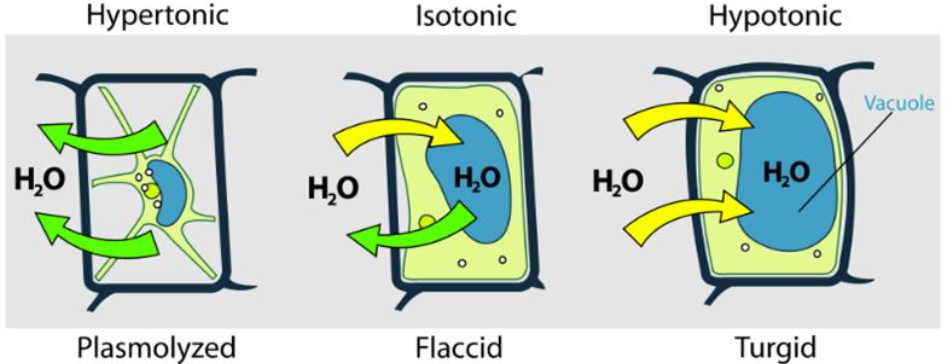
\includegraphics[width=35mm]{src/Images/osmosis.png}
        Hypertronic: high solute concentration\\
        Hypotonic: low solute concentration.\\
\end{minipage}

Membrane is \textbf{selectively permeable}, allowing some molecules to pass through while blocking others.\\

\textbf{Facilitated Diffusion:}\\
\begin{minipage}{0.42\linewidth}
    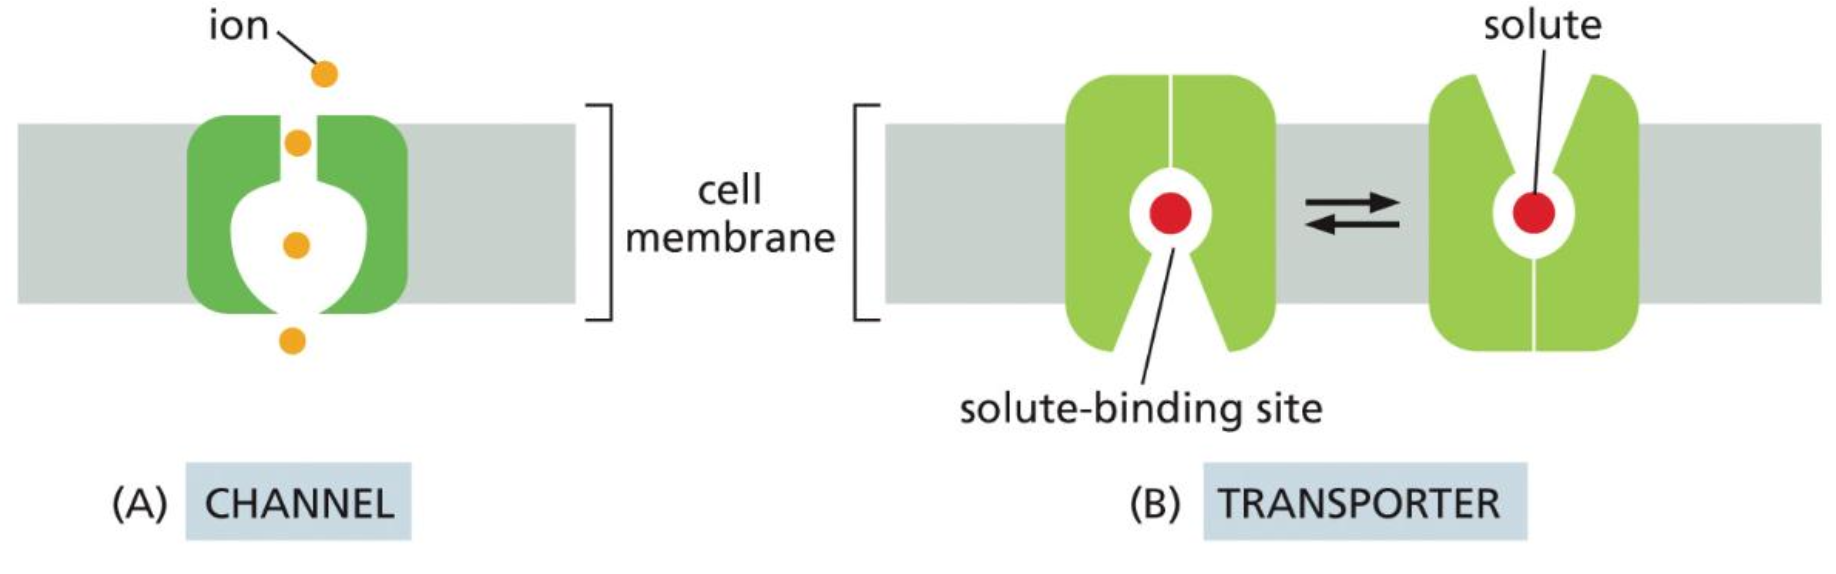
\includegraphics[width=35mm]{src/Images/channel.png}
\end{minipage}
\begin{minipage}{0.58 \linewidth}
    \begin{itemize}
        \item selective to size and charge of solute
        \item bidirectional
        \item gated by external inputs
        \item Transporter good for large molecules
    \end{itemize}
\end{minipage}